\chapter{The Accretion Disk: Novikov--Thorne and Page--Thorne}
\label{ch:disk}

\section{The Novikov--Thorne disk and the Page--Thorne flux}
\label{sec:pagethorne}

The accretion flow is modelled as the geometrically thin, optically thick
equatorial disk of \citet{NovikovThorne1973}, using the closed-form
time-averaged flux profile of \citet{PageThorne1974}, their eq.~(15n): in
terms of $x = \sqrt{r/M}$ and the roots $x_{1,2,3}$ of
$x^3 - 3x + 2a_* = 0$,
\begin{align}
F(r) \propto{}& \frac{1}{x^4\left(x^3 - 3x + 2\astar\right)}
\Big[x - x_0 - \tfrac{3}{2}\astar\ln\frac{x}{x_0} \nonumber\\
&{}- \sum_{i=1}^{3}
\frac{3(x_i-\astar)^2}{x_i(x_i-x_j)(x_i-x_k)}
\ln\frac{x-x_i}{x_0-x_i}\Big],
\label{eq:pagethorne}
\end{align}
with $x_0 = \sqrt{r_{\rm ISCO}/M}$ (implemented by \texttt{flux} in
\texttt{physics/src/disk\_model.cpp}). Two numerical notes: the root
$x_2 \to 0$ as $\astar \to 0$ and its logarithm coefficient must be
guarded at the Schwarzschild limit; and the far-field expansion is
\emph{not} the Newtonian $1-\sqrt{r_{\rm in}/r}$ profile --- the GR log
terms shift the constant, $f(x) \to x - c + 3/x + \mathcal{O}(x^{-2})$
with $c \simeq 3.976$ for $\astar = 0$, which the unit tests assert
against the exact expansion rather than the Newtonian folklore form.
The profile is evaluated between $r_{\rm ISCO}$ and an outer radius
$r_{\rm out}$.

\stub{The thin-disk conservation laws (mass, energy, angular momentum)
leading to the radial structure; the full $f(x)$ derivation with the
$x_1, x_2, x_3$ roots and log terms. New figures: $F(r)$ and $T(r)$
profiles at several $\astar$ (needs \texttt{physics\_tables}).}

\section{Redshift factor and Doppler beaming}
\label{sec:gfactor}

Each backward-traced ray that crosses the equatorial annulus is assigned
the redshift factor
\begin{equation}
g \equiv \frac{\nu_{\rm obs}}{\nu_{\rm emit}}
      = \frac{\sqrt{-(g_{tt} + 2\Omega g_{t\phi} + \Omega^2
        g_{\phi\phi})}}{1 - \Omega\,b_\gamma},
\label{eq:gfactor}
\end{equation}
where $\Omega$ is the circular-orbit angular velocity at the crossing
radius and $b_\gamma = L_z/E$ the photon's impact parameter. Since a
blackbody redshifted by $g$ is exactly a blackbody at temperature $gT$, the
observed bolometric intensity scales as $g^4$ (Doppler beaming,
\texttt{bolometric} in \texttt{disk\_model.cpp}), and the colour follows
from the Planck spectrum at $g\,T_{\rm eff}(r)$ through the CIE 1931
observer (\texttt{blackbody\_rgb}). Photon sub-rings are labelled by the
number $n$ of equatorial crossings prior to the terminating one
\citep{Johnson2020}; their metrology is the subject of
Chapter~\ref{ch:ring}.

\stub{Derivation of the $g^4$ law from Liouville invariance of
$I_\nu/\nu^3$; the Planck-to-CIE colour pipeline. New figures: $g$-factor
image map; blackbody/CIE locus.}

\section{The rendered disk}
\label{sec:diskrender}

Fig.~\ref{fig:disk} shows the Novikov--Thorne disk at $\astar = 0.94$,
$i = 80\degr$. The redshift factor spans $g = \GMin$ to $\GMax$ across the
image, and the resulting $g^4$ beaming makes the approaching side
$\BeamRatio\times$ brighter in bolometric flux than the receding side ---
the classic one-sided appearance anticipated by \citet{Luminet1979} and
rendered cinematically by \citet{James2015}.

\begin{figure}
\centering
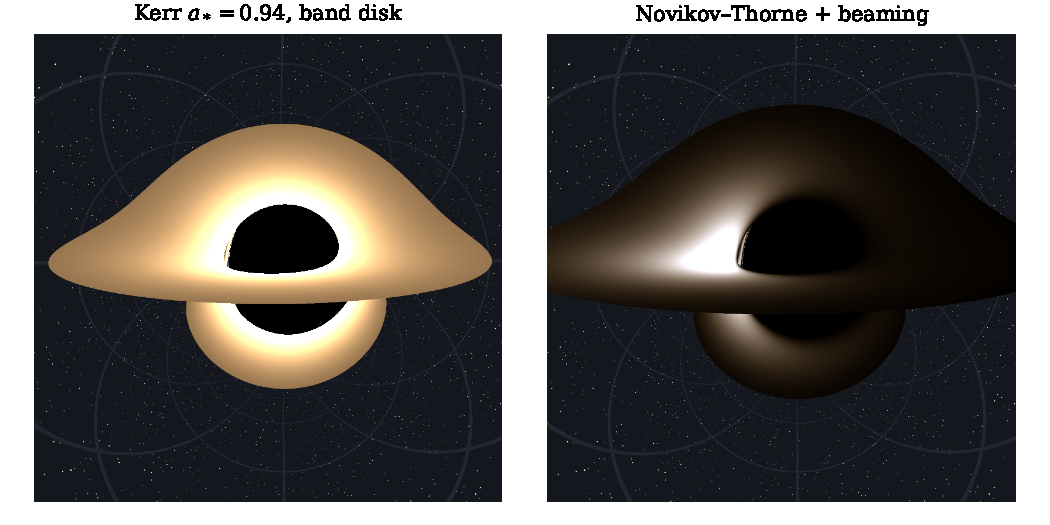
\includegraphics[width=0.85\textwidth]{figures/fig_disk_render.pdf}
\caption{CPU reference render of the Novikov--Thorne disk at
$\astar=0.94$, $i=80\degr$ (linear sRGB from Planck spectra at
$g\,T_{\rm eff}$). Doppler beaming brightens the approaching limb by a
bolometric factor of \BeamRatio.}
\label{fig:disk}
\end{figure}

\section{Spin morphology of the disk image}
\label{sec:spinmorphology}

\stub{User-requested topic (THESIS\_PLAN Part 1c): at $\astar = 0$ the
wound streamlines of the display layer form smooth, continuous,
near-concentric lines around the whole disk; at high spin
($\astar \approx 0.906$) the coherent bright streamlines collapse to a
small patch on the approaching side --- the ISCO moves inward, frame
dragging and $g^4$ beaming intensify and asymmetrise. Awaiting the user's
two comparison engine renders; captions will carry the exact
\texttt{sgr\_engine} command line that regenerates each.}
